\section{Ease of use and developer productivity}\label{usability}
We describe our experiences in implementing and running the TPC-DS Benchmark in Databricks and EMR Presto. Our description is complemented by observations about the usability of the two systems and its associated tools, which can have a significant effect on developer productivity. We point out beforehand, however, that these aspects can be influenced by the skills and previous experience, the preferences, and the usual practices of individual developers. Furthermore, it is not possible to cover all of their features in a relatively limited study.

For ease of presentation, for each main aspect we describe first the features of Databricks, subsequently we do the same for EMR Presto, providing additional commentaries discussing how the two compare.

\subsection{General features}
\subsubsection{Databricks Unified Analytics Platform}
As its name suggests, Databricks provides a unified platform to perform Big Data analytics. The entry point for this platform is the web GUI, shown in Figure \ref{fig:databricksMainGUI}.

\begin{figure}
   \begin{center}
   \scalebox{0.85}{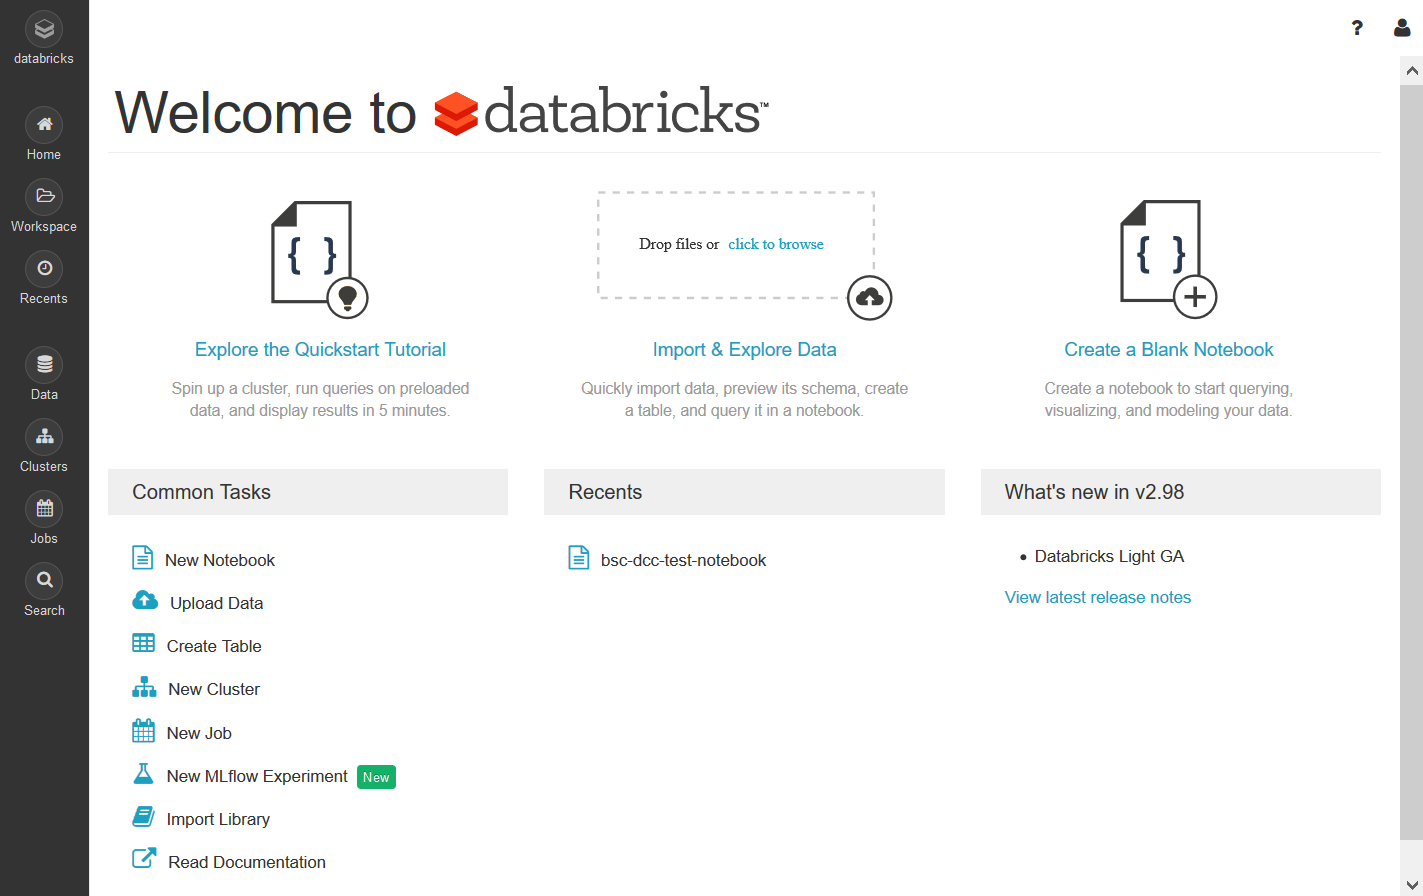
\includegraphics[width=7.0in]{imgs/usability/DatabricksMain.png}}
   \end{center}
   \caption{Databricks main web GUI.}
   \label{fig:databricksMainGUI}
\end{figure}

It is desirable to keep the main components of data analytics processes logically separate but easily accessible. We consider these components to be the applications or program logic, the data, and the computational resources, i.e. clusters. Regarding the first, data analytics tasks in Databricks can be started mainly from notebooks and jobs. Notebooks can be accessed through the Workspace while jobs can be created via a web application or a REST API. In addition, Databricks also provides a JDBC interface for SQL, which we cover in Section \ref{databricksJDBC}.

In relation to data, Databricks provides the facilities to visualize databases, tables and their comprising columns, and samples of the data. We depict the corresponding interface in Figure \ref{fig:databricksDataCatalogGUI}. This catalog is supported by an underlying AWS RDS MySQL Hive-compatible metastore.

\begin{figure}
   \begin{center}
   \scalebox{0.85}{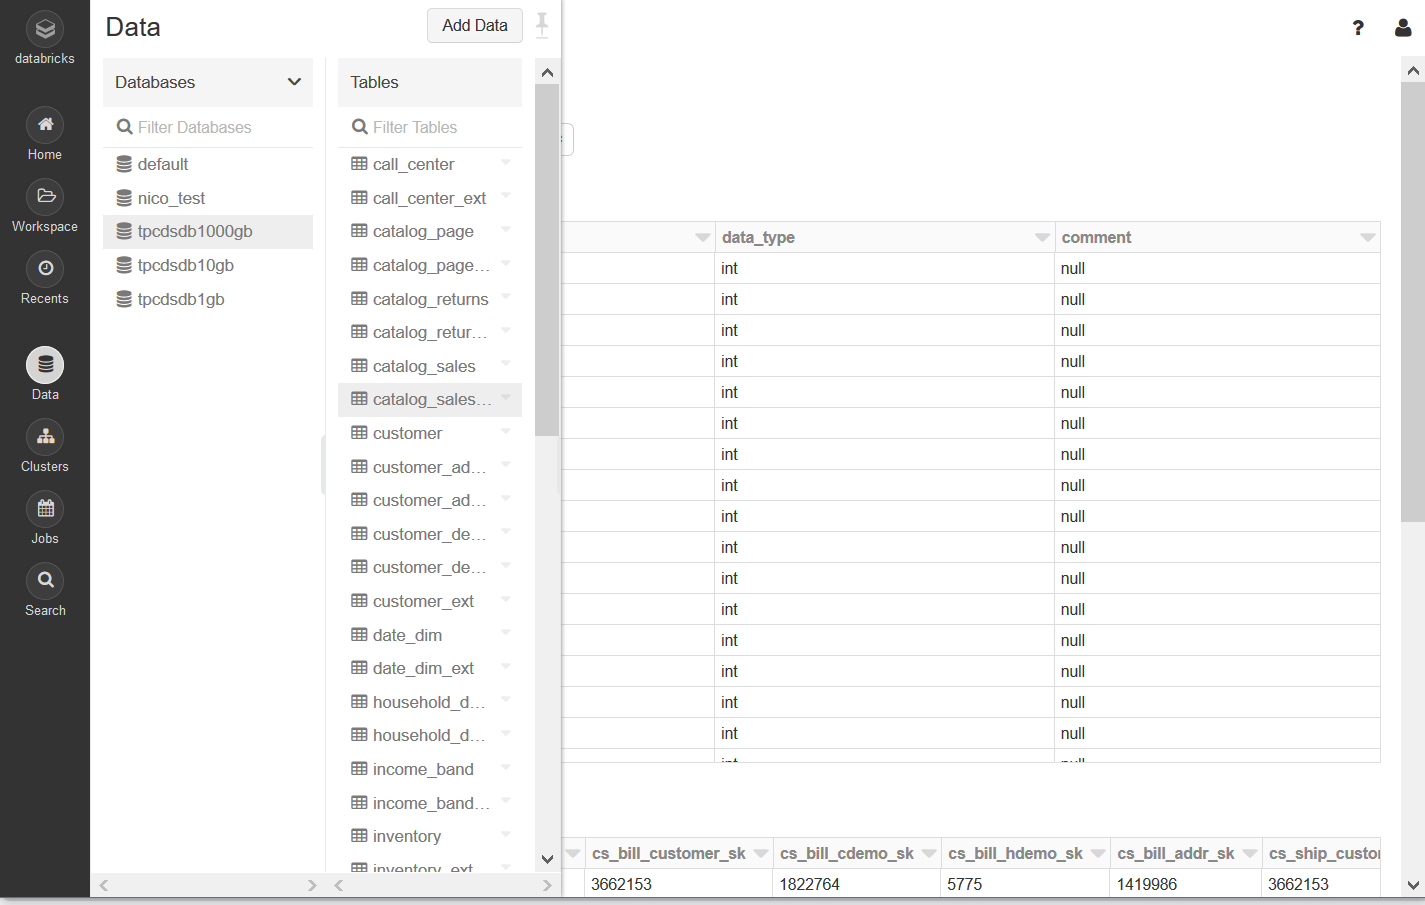
\includegraphics[width=7.0in]{imgs/usability/DatabricksData.png}}
   \end{center}
   \caption{Databricks data catalog web GUI.}
   \label{fig:databricksDataCatalogGUI}
\end{figure}

Clusters in Databricks take one of two forms, Interactive and Job clusters. The first support notebooks, while the second are created to execute a predefined job and destroyed after its completion. This is an important feature since with a Job cluster the total cost can be minimized, provided the application ran by the Job is developed accordingly.

An important consideration for clusters for Big Data analytics is being able to easily and quickly to configure them, including the hardware resources and the software deployed. Figure \ref{fig:databricksClusterCreationGUI} shows the web GUI that Databricks provides for this task.

\begin{figure}
   \begin{center}
   \scalebox{0.85}{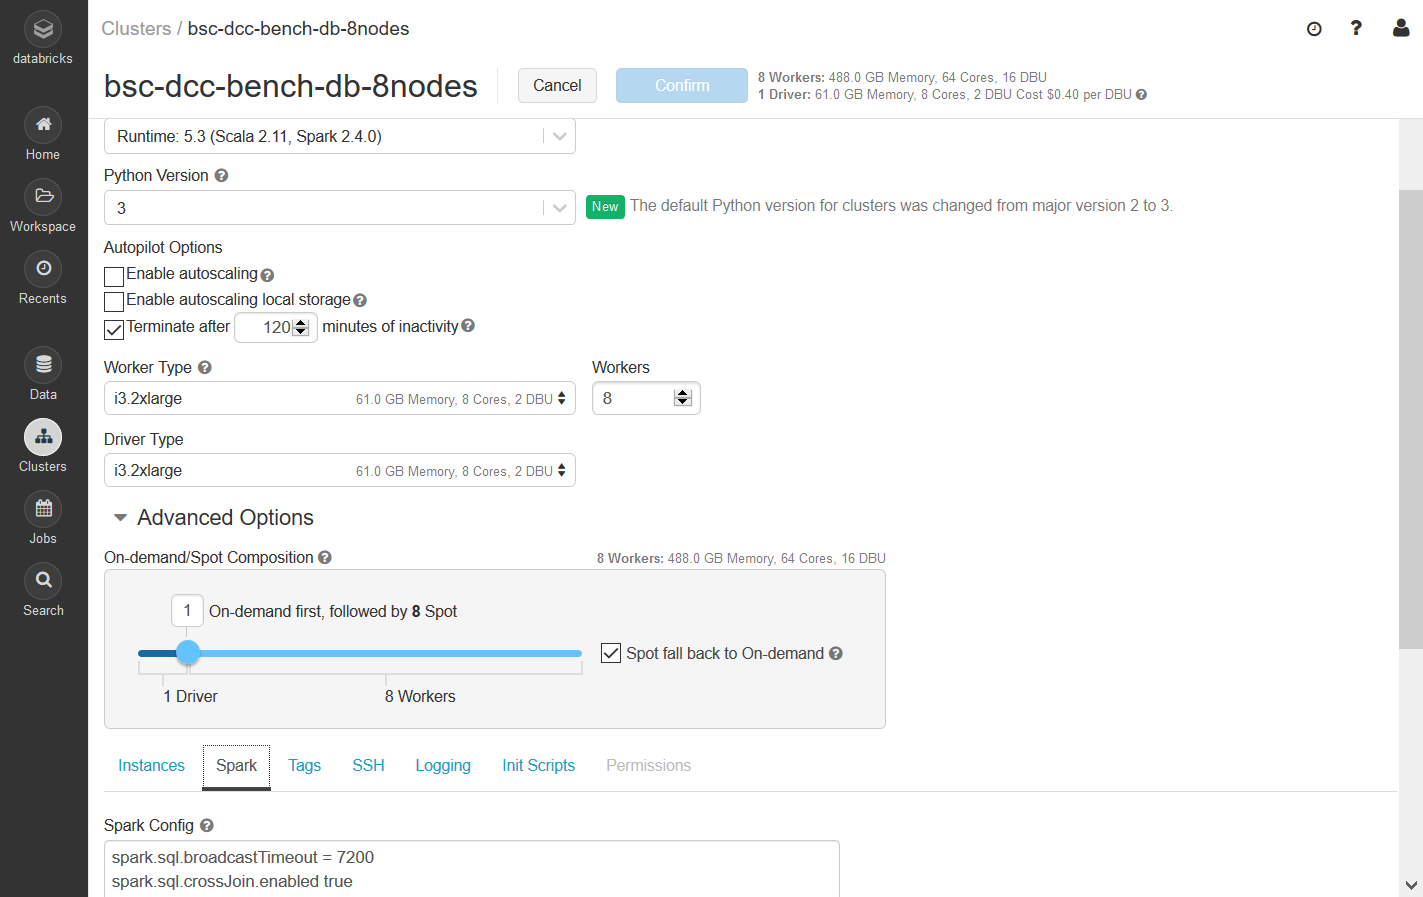
\includegraphics[width=7.0in]{imgs/usability/DatabricksClusterCreation.png}}
   \end{center}
   \caption{Databricks cluster creation web GUI.}
   \label{fig:databricksClusterCreationGUI}
\end{figure}

It is easy to select essential properties of the cluster such as the Runtime and the type of EC2 instances, as it is to be expected. More relevant to our discussion, it is possible to specify configuration properties for Spark and an SSH key for command line access. In the case of Interactive clusters, once they have been created and are online, they can be associated with a notebook or with a job to enable them to run.

Essentially, Databricks covers the main aspects of applications, data, and clusters adequately. It provides easy and fast access to each and works toward making their interoperation transparent for the user. While its design principles are commendable, at the level of applications some issues arise, which we address in Subsection \ref{runningApplicationsDatabricks}.

\subsubsection{AWS EMR Presto}
We find in Figure \ref{fig:emrMainGUI} the Web GUI entry point for EMR, which includes Presto among its supported Big Data frameworks. This GUI is embedded within the AWS portal and gives fast access to past cluster configurations that can be cloned and modified as desired to create new clusters. We discuss first the cluster creation process with EMR and then address data management and running applications.

\begin{figure}
   \begin{center}
   \scalebox{0.85}{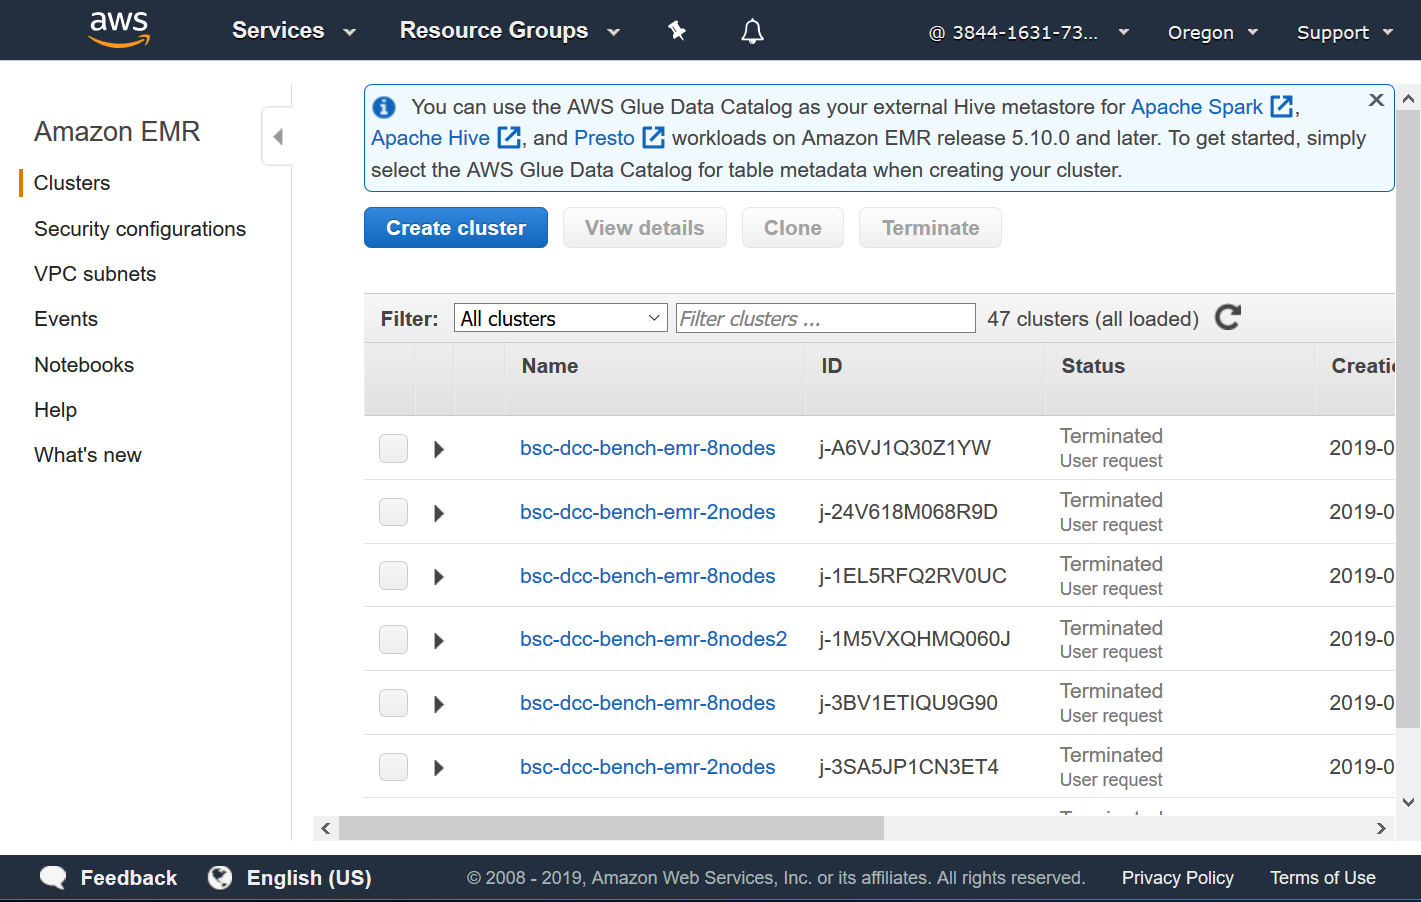
\includegraphics[width=7.0in]{imgs/usability/EMRmain.png}}
   \end{center}
   \caption{AWS EMR main  web GUI.}
   \label{fig:emrMainGUI}
\end{figure}

Figure \ref{fig:emrClusterCreationGUI} depicts the cluster creation process for EMR. Again, multiple Big Data processing frameworks are supported. In this example, Presto is selected along with additional software that in our experiments would be available but not used. Importantly, AWS Glue is selected to be used for the Hive-compatible metastore for Presto. A single text input is used to provide software configurations, since multiple systems are involved, a series of predefined JSON attribute names enable to distinguish among them.

\begin{figure}
   \begin{center}
   \scalebox{0.85}{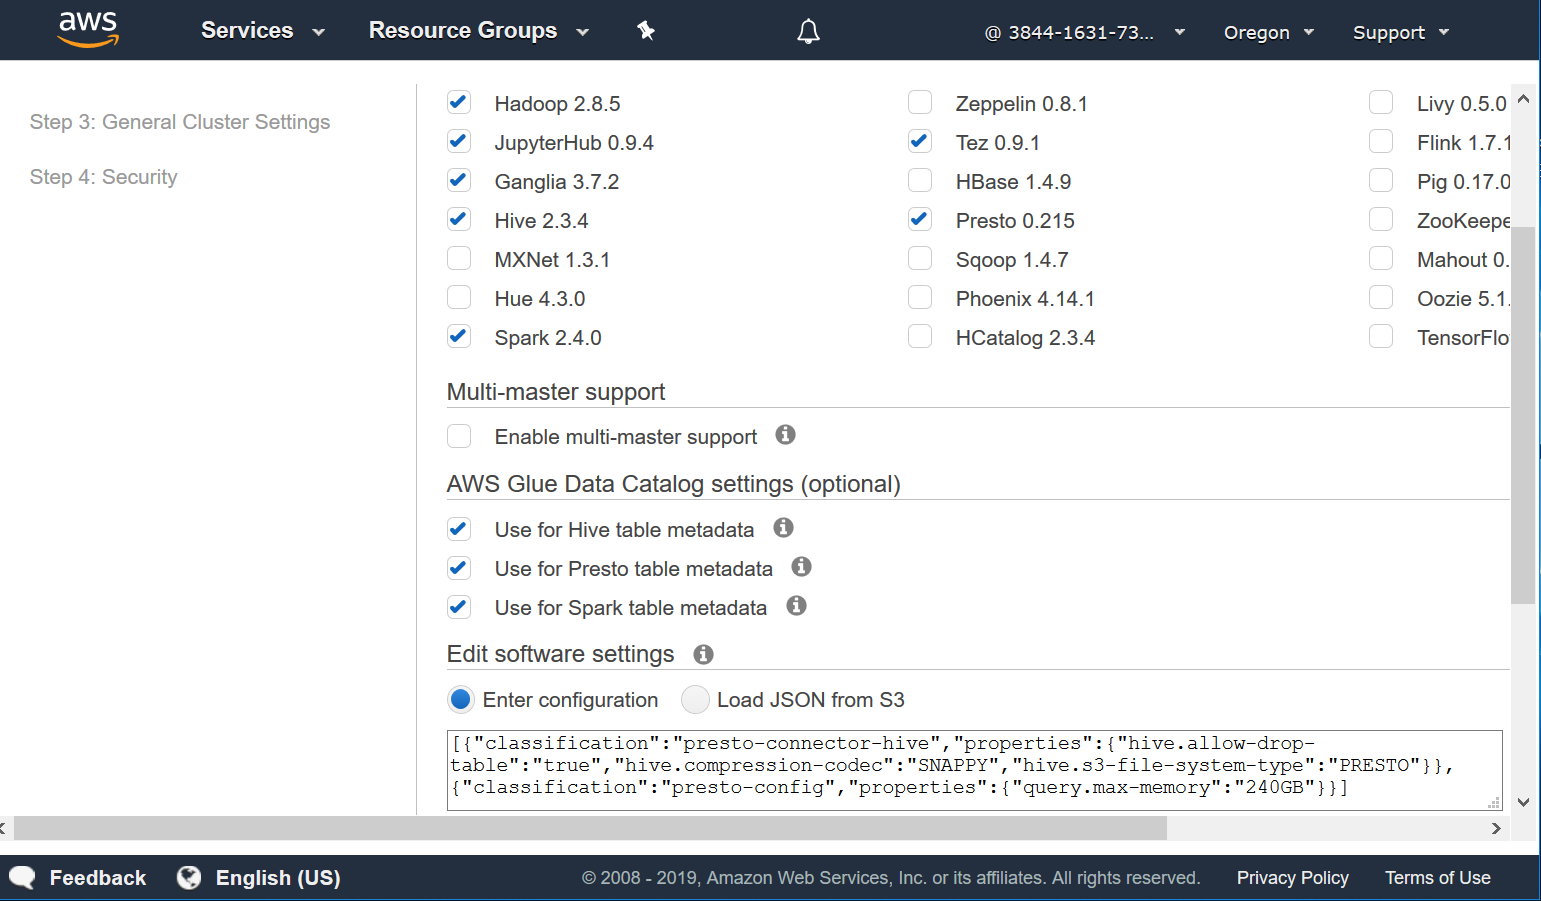
\includegraphics[width=7.0in]{imgs/usability/EMRclusterCreation.png}}
   \end{center}
   \caption{AWS EMR cluster creation web GUI.}
   \label{fig:emrClusterCreationGUI}
\end{figure}

It is a significant benefit to be able to configure the software frameworks in this manner. Especially given that doing so for Presto by means of an alternative initialization bash script is quite an error-prone and complex task, due to the delays in the creation of the configuration files. We also note that, in our experience, changing the configuration afterwards and restarting the cluster failed to achieve the desired effects in some cases.

In regards to the creation of clusters, both Databricks and EMR Presto offer similar advantages.

As mentioned earlier, we use AWS Glue for the metastore used by EMR Presto. AWS Glue is designed to be an integrated data catalog independent of the location of the data sources. It is serverless, persistent, and can be used by Presto without additional configuration with any newly created EMR cluster. As Figure \ref{fig:awsGlueGUI} shows, its accompanying web GUI enables to visualize and edit databases, tables and their component columns, and their related metadata.

\begin{figure}
   \begin{center}
   \scalebox{0.85}{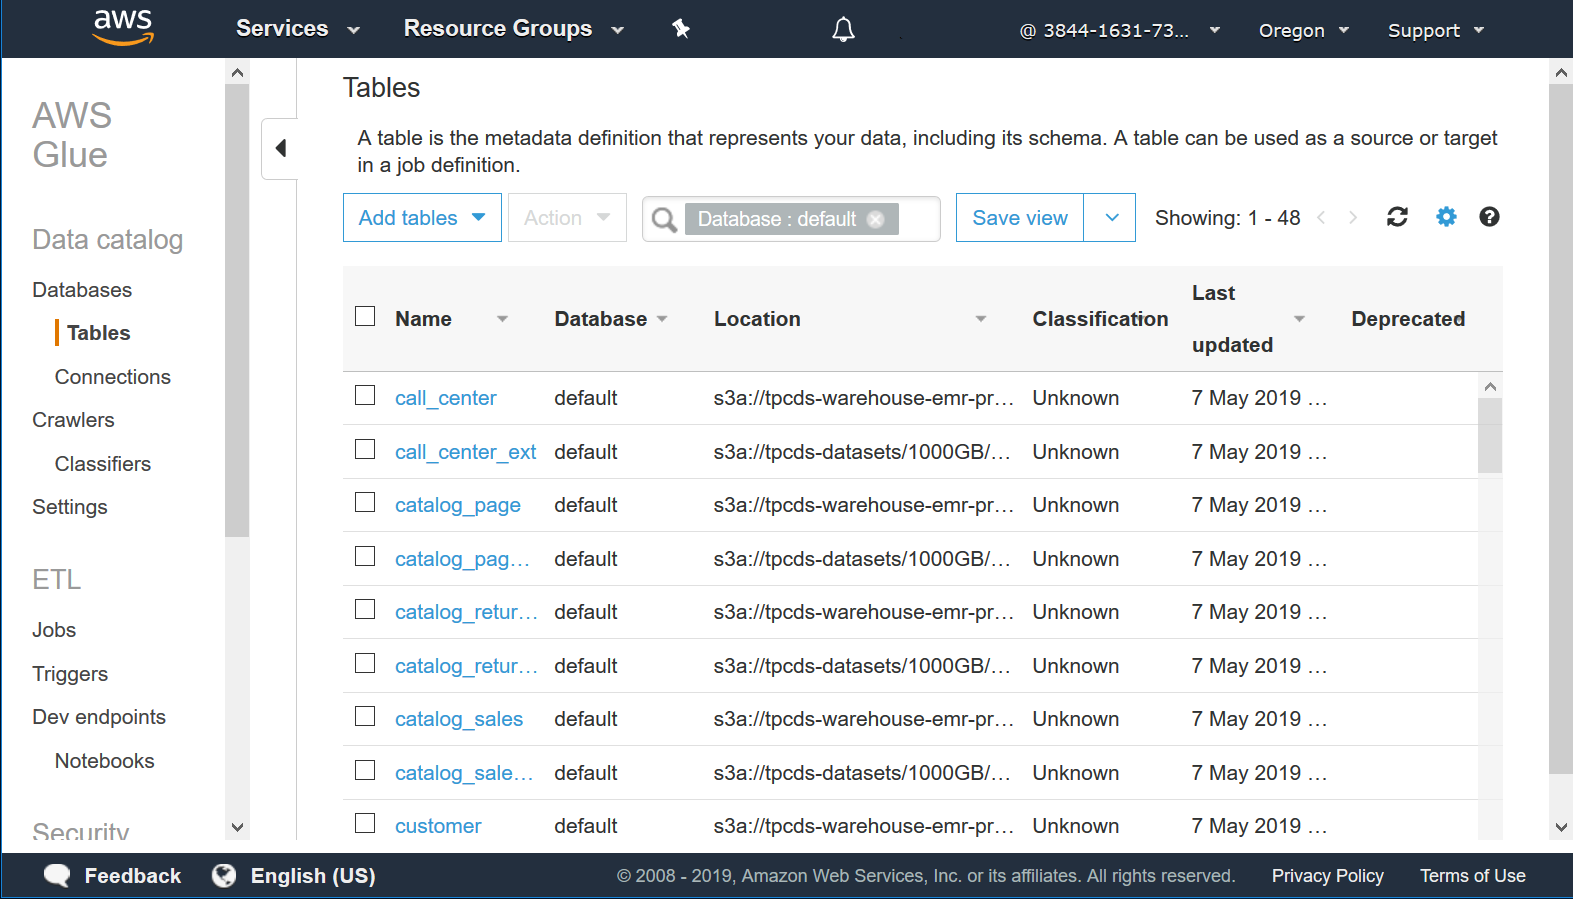
\includegraphics[width=7.0in]{imgs/usability/AWS_Glue.png}}
   \end{center}
   \caption{AWS Glue web GUI.}
   \label{fig:awsGlueGUI}
\end{figure}

In principle, EMR Presto with AWS Glue offers comparable capabilities to Databricks for data management, keeping an independent catalog and offering capabilities to explore it. However, as we discuss in Section \label{referenceResultsDataLoading}, AWS Glue does not support column statistics, which is a major drawback.

In relation to application development, EMR Presto offers two main interfaces: JDBC and a REST-based CLI. We compare these in Section \label{prestoJDBvsCLI}, determining that although they have a similar performance, the ability of keeping the connection alive with JDBC can be advantageous for some applications. EMR Presto can also be used with Zeppelin notebooks, since, as we can see in Figure \label{fig:emrClusterCreationGUI}, Zeppelin is an optional software component of EMR, and a JDBC connector enables their interoperability. However, we did not evaluate this capability. We can conclude that EMR Presto offers similar capabilities for application development to those of Databricks, with the exception that EMR Presto does not have a feature comparable to the Jobs API and GUI of Databricks. To a large extent this can be explained by the fact that Presto is a SQL engine, used either in a stand-alone manner or to execute embedded SQL queries through a programming language. In contrast, Databricks provides a unified programming model supported by Spark, and therefore closely related to the Java and Scala platforms.

In summary, both EMR Presto and Databricks offer good features in relation to data management, application development, and cluster creation and configuration. No major gaps in terms of functionality are present in either system. Nevertheless, Databricks offers a more unified and better integrated platform. Some of these advantages are clearer when analyzing closely the execution of applications, as we do in the next subsection.

\subsection{Running applications}
\subsubsection{Databricks Unified Analytics Platform}\label{runningApplicationsDatabricks}

As mentioned earlier, Databricks offers notebooks and a Job API as the main means of running applications. We present the web GUI of a notebook in Figure \ref{fig:databricksNotebookGUI}.

\begin{figure}
   \begin{center}
   \scalebox{0.85}{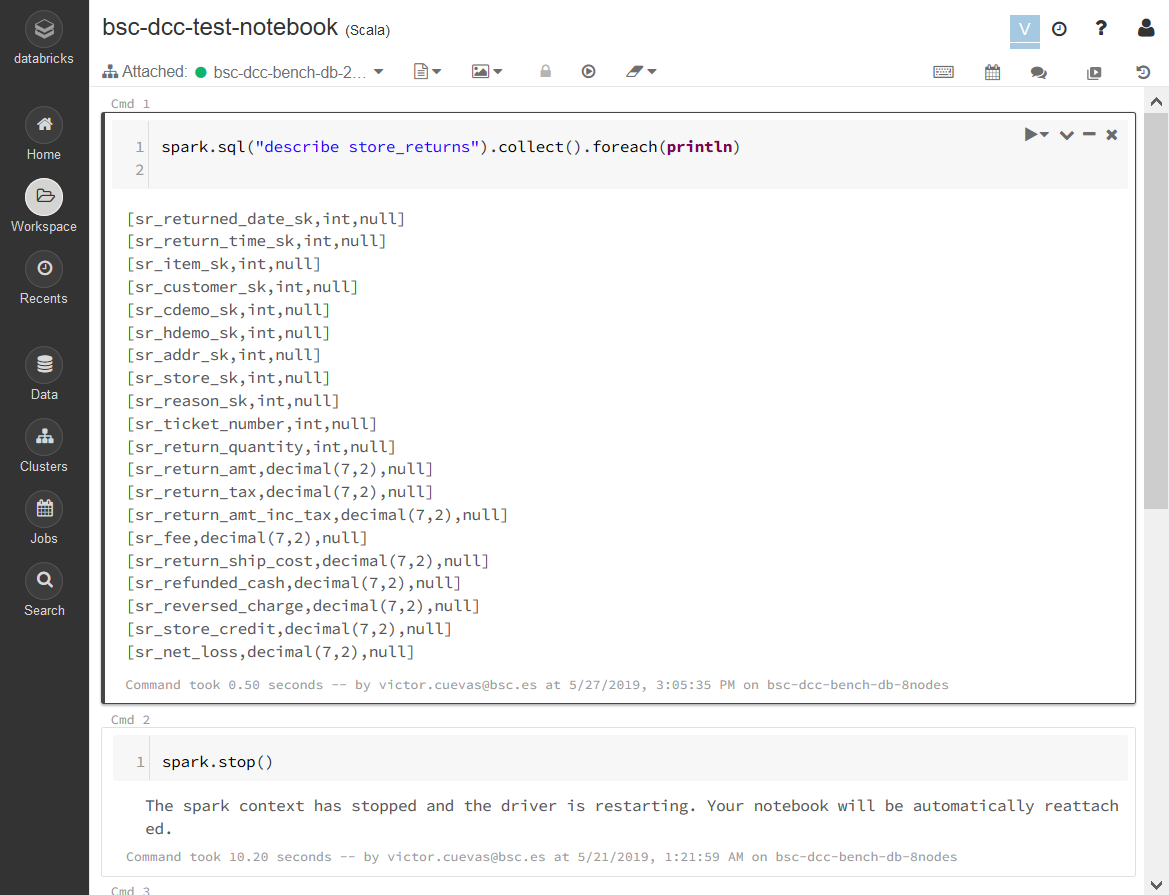
\includegraphics[width=7.0in]{imgs/usability/DatabricksNotebook.png}}
   \end{center}
   \caption{Databricks web GUI for notebooks.}
   \label{fig:databricksNotebookGUI}
\end{figure}

A notebook allows executing a series of commands running on a cluster it is attached to. It provides several advantages over a command line interface. It is easier to use, persistent, editable, shareable, tasks can be executed sequentially or individually, etc. Although this kind of platform is not adequate for a benchmarking application, it did enable us to test and debug several commands and SQL statements. Particularly important in our context is the execution of SQL statements by means of the spark session object, for which Figure \ref{fig:databricksNotebookGUI} presents an example.

To run production applications users have at their disposal the Jobs API, which can be accessed via REST or through a web GUI, the latter shown in Figure \ref{fig:databricksJobsGUI}.

\begin{figure}
   \begin{center}
   \scalebox{0.85}{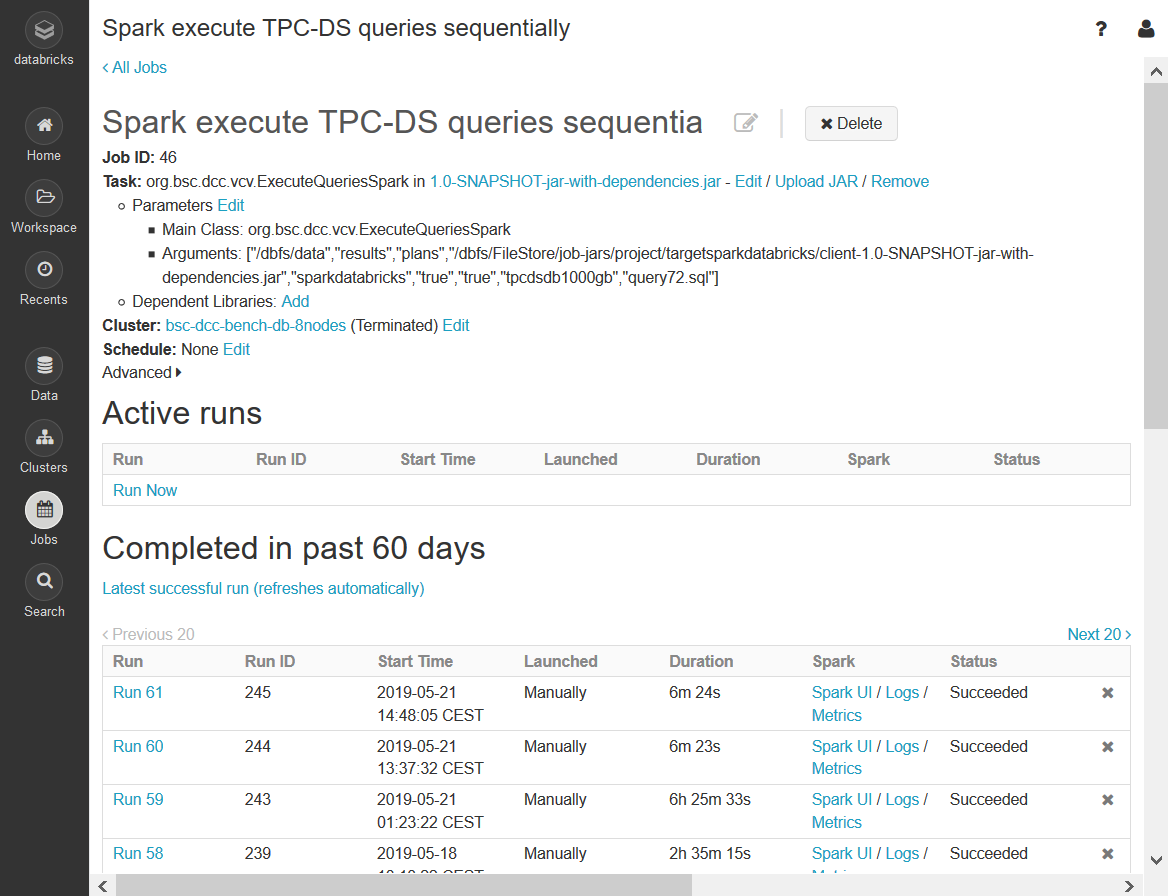
\includegraphics[width=7.0in]{imgs/usability/DatabricksJob.png}}
   \end{center}
   \caption{Databricks Jobs web GUI.}
   \label{fig:databricksJobsGUI}
\end{figure}

As we can see, a Job consists of a Task associated with a jar file, a series of parameters, and additional libraries (consisting of jar files also). It can be executed by associating it with a cluster. Active runs can be monitored and past runs can be examined. This feature greatly facilitates auditing, debugging, and to some extent recovering the provenance of application results.

Our TPC-DS Benchmark implementation for Databricks is based on three separate jobs for the Data Loading Test, the Power Test, and the Throughput Test. An additional application was developed to create the table and column statistics. In all cases, a single jar file incorporates the Java code and the SQL statements. The code extracts the SQL statement files from the jar, transforms them if necessary, and executes them via the spark session object, keeping track of execution times, evaluation plans, and results.

These applications are based on a prototype developed and tested on a Docker deployment of open source Apache Spark, in which jar files are executed via spark-submit. To run them on Databricks, once the corresponding jar file is created via the Maven compilation process, a job can be created via the Jobs REST API employing simple bash scripts that use the curl command. From the web GUI, the new Job can be attached to an existing or new cluster and executed.

We would like to point out that migrating the TPC-DS benchmarking application to Databricks was relatively straightforward. Nevertheless, some issues did emerge that required attention and that could pose significant obstacles for application developers, especially if moving from open source Spark to Databricks.

First, one of the aspects to consider in migrating the application is the metastore. In our prototype we used PostgreSQL 10.6 running on Docker and configured the system to use it via the hive-site.xml file and the spark-defaults.conf file. In particular, we added to the latter file the parameter spark.sql.hive.metastore.version 2.3.0. Trying to use this configuration parameter triggered errors traced back to the fact that the Databricks 5.3 Runtime provides a default Hive-compatible metastore with version 0.13.0. Although this may appear very restrictive, the 0.13.0 version already includes the main characteristics needed for data analytics.

The default metastore is implemented to be transparent so accessing it for a manual schema and version upgrade is difficult. However, adapting an external metastore from a more recent version is possible. The best alternative is to simply use the default metastore and switching to an external one only if truly necessary.

A second issue appeared with the use of the spark session object on a multi-threaded environment. The session object is the entry point for programming an application with Apache Spark, and this applies to notebooks as well, as seen in the example of Figure \ref{fig:databricksNotebookGUI}. For a Java application, accessing this object usually implies an instruction of the form:

\vspace{0.5cm}
\noindent this.spark = SparkSession.builder().getOrCreate();
\vspace{0.5cm}

For single-threaded tasks like data loading or sequential query execution for the Power Test, this presented no issues on our prototype or on Databricks. It also worked for a multi-threaded task like concurrent query processing for the Throughput Test in our prototype application, by sharing a reference to the same session object among the different threads. However, this approach running on Databricks resulted in the rather
obscure error:

\vspace{0.5cm}
\noindent org.apache.spark.sql.AnalysisException: Undefined function: 'sum' 
\vspace{0.5cm}

Analyzing the Spark source code led to an alternative way of accessing the Spark session object within a thread that avoided errors:

\vspace{0.5cm}
\noindent Option \textless SparkSession\textgreater \ opt = SparkSession.getDefaultSession();\\
SparkSession session = opt.getOrElse(null);
\vspace{0.5cm}

Another issue related to the spark session object is that when the application code stops the session when the application terminates, i.e., with an instruction like spark.stop(), this causes the status of the job to be reported as Failed, as shown in Figure \ref{fig:databricksJobsFailed}.

\begin{figure}
   \begin{center}
   \scalebox{0.85}{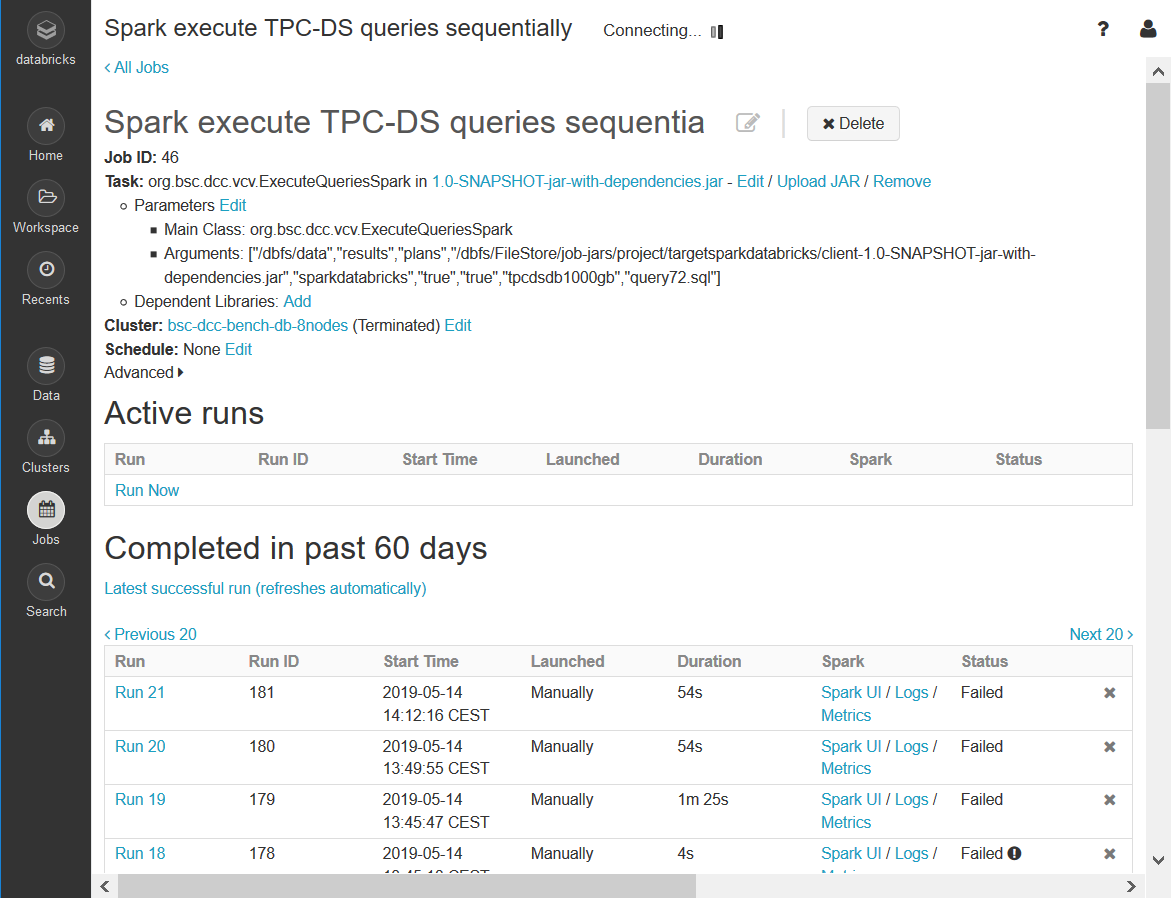
\includegraphics[width=7.0in]{imgs/usability/DatabricksJobFailed.png}}
   \end{center}
   \caption{Jobs marked as Failed in the web GUI.}
   \label{fig:databricksJobsFailed}
\end{figure}

Removing the instruction that closes the session changed the Status of the completed jobs to Succeeded. However, not closing the session can have undesirable effects in some cases. For instance, in our application the log4j logs do not roll over, meaning new files are not created for each execution if the session is not closed. If we stop the session through a notebook the state of the runtime is reset and the logs roll over as desired.

In summary, adapting an existing open source Spark application to Databricks is relatively easy. Nevertheless, special consideration needs to be taken in some cases to deal with unexpected behaviors and limitations.

An additional aspect that is very important to running data analytics applications is having a distributed file system, which allows access and storage of large files across the cluster. Databricks provides for this purpose the Databricks File System (DBFS), which comes equipped with a CLI, a REST API, and a programmatic interface for Python and Scala.

DBFS is readily available in any Databricks cluster and mounted within the file system, therefore files in DBFS can be accessed and manipulated as local files. The DBFS storage is not tied to a particular cluster, it is persisted by S3 so it is not lost after clusters are destroyed. Furthermore, user AWS S3 buckets can also be mounted through DBFS using a FUSE mounting point. Even if it is not used for data files, like in our case since we use S3 directly (except for the preliminary experiments in Section \ref{preliminaryExperiments}), it is still very useful to save SQL query files, log files, and jar files for Databricks jobs.

\subsubsection{AWS EMR Presto}

As stated earlier, the main methods of accessing the EMR Presto server are a JDBC client, and a CLI built around a REST API. Our prototype benchmarking application for Presto was developed in Java, running within a Docker container and submitting queries to a Presto server similarly deployed within a Docker container. In order to minimize latency, we decided to deploy this Docker-based application on the master node of the EMR cluster.

Deploying and running our Docker-based Java application to the EMR cluster node was straightforward. Aside from modifying the JDBC URL, no changes to the EMR Presto configuration were required to run our application. This is to be expected with a JDBC compliant application and in fact, this same application (although running without Docker) was able to access Databricks through JDBC with minimal changes, relying on the URL provided in the cluster creation web GUI.

EMR Presto does not provide a feature analogous to the Jobs API and web GUI of Databricks. However, this is understandable given the service-based architecture of Presto and the fact that it is limited to a SQL engine. A programmatic interface like the Spark session object on Databricks may not be appropriate in this context. Since the functionality itself is clearly delimited, i.e., executing SQL statements, the advantages of exclusively having a standardized interface like JDBC and REST for interoperability can outweigh the ease of application development through a closely linked programmatic interface.

Databricks, on the other hand, offers much more functionality supported by Spark, which is designed to be a common framework for different types of data analytics. A programmatic interface therefore facilitates building specialized data analytics applications for developers. A disadvantage in this case is that the application code becomes dependent on that interface.

In terms of a distributed file system, EMR Presto employs HDFS on top of Amazon Elastic Block Store (EBS) or the associated NVMe SSDs. However, in either case HDFS is dependent on the EC2 instances associated with the cluster so it is lost when the cluster is destroyed.

\subsection{Monitoring applications}

\subsubsection{Databricks Unified Analytics Platform}

The web GUI of Databricks adapts the open source Apache Spark web GUI; we depict it in Figure \ref{fig:databricksSparkGUI}.

\begin{figure}
   \begin{center}
   \scalebox{0.85}{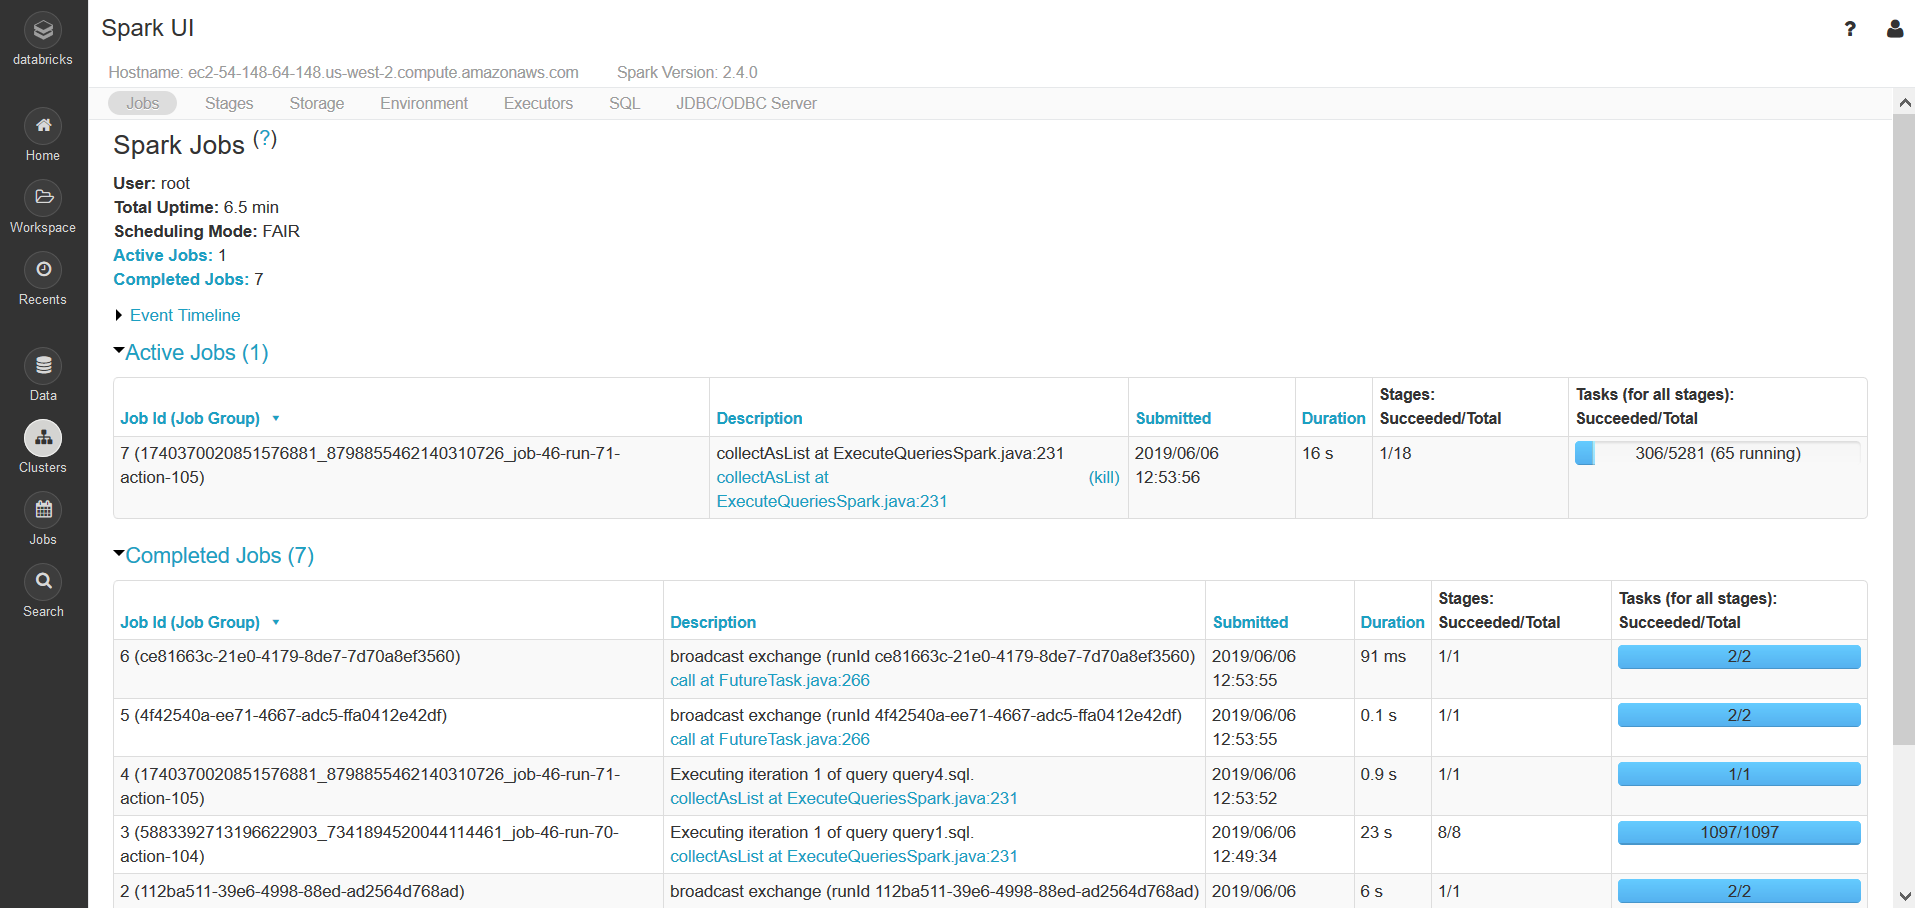
\includegraphics[width=7.0in]{imgs/usability/DatabricksSparkGUIJobs.png}}
   \end{center}
   \caption{Databricks Spark web GUI.}
   \label{fig:databricksSparkGUI}
\end{figure}

A list of the various jobs running and their progress can be viewed from this interface. Each of these jobs comprises a series of stages; these can be displayed by selecting the corresponding job as shown in Figure \ref{fig:databricksSparkGUIDAG}.

\begin{figure}
   \begin{center}
   \scalebox{0.85}{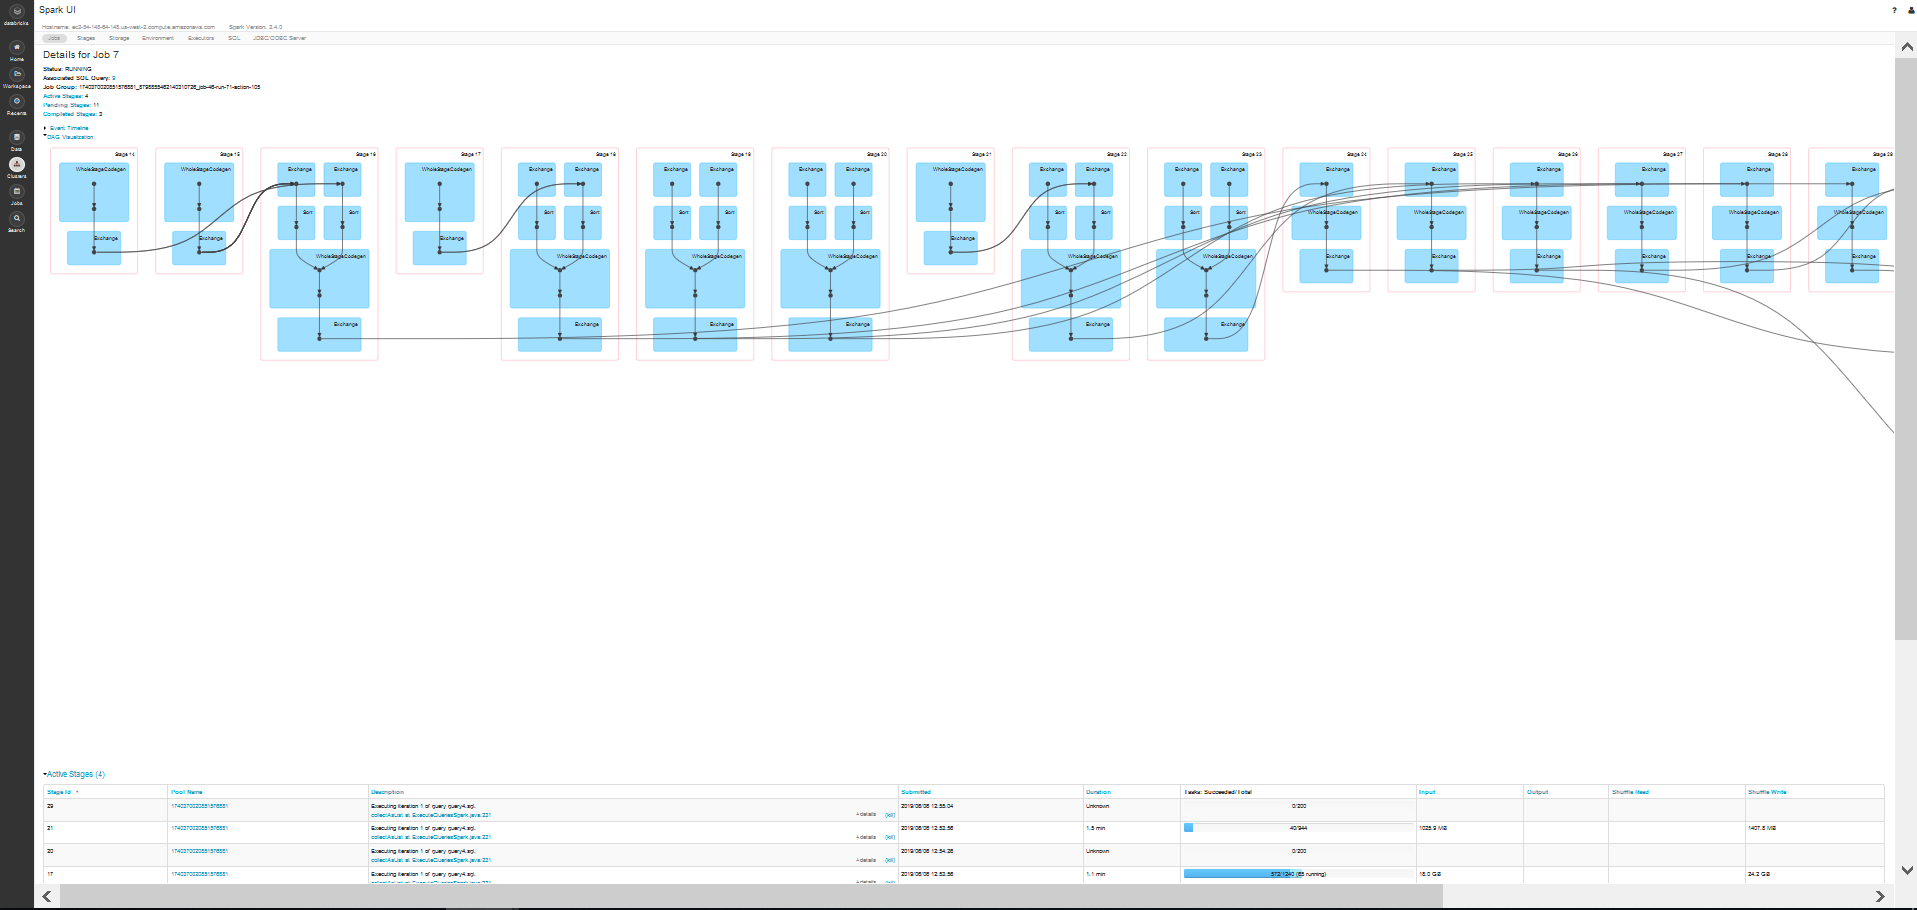
\includegraphics[width=7.0in]{imgs/usability/DatabricksSparkGUIDAG.png}}
   \end{center}
   \caption{Databricks Spark stages visualization.}
   \label{fig:databricksSparkGUIDAG}
\end{figure}

A visualization of the DAG (directed acyclic graph) of the various stages associated with the job is provided. For queries, it represents the implementation of the query evaluation plan, although visually it can be hard to follow. Fortunately, a custom visualization for SQL queries is also available, it is depicted in Figure \ref{fig:databricksSparkGUISQL}. It significantly facilitates understanding a query evaluation plan, by both the improved DAG and the annotations on the various operators.

\begin{figure}
   \begin{center}
   \scalebox{0.85}{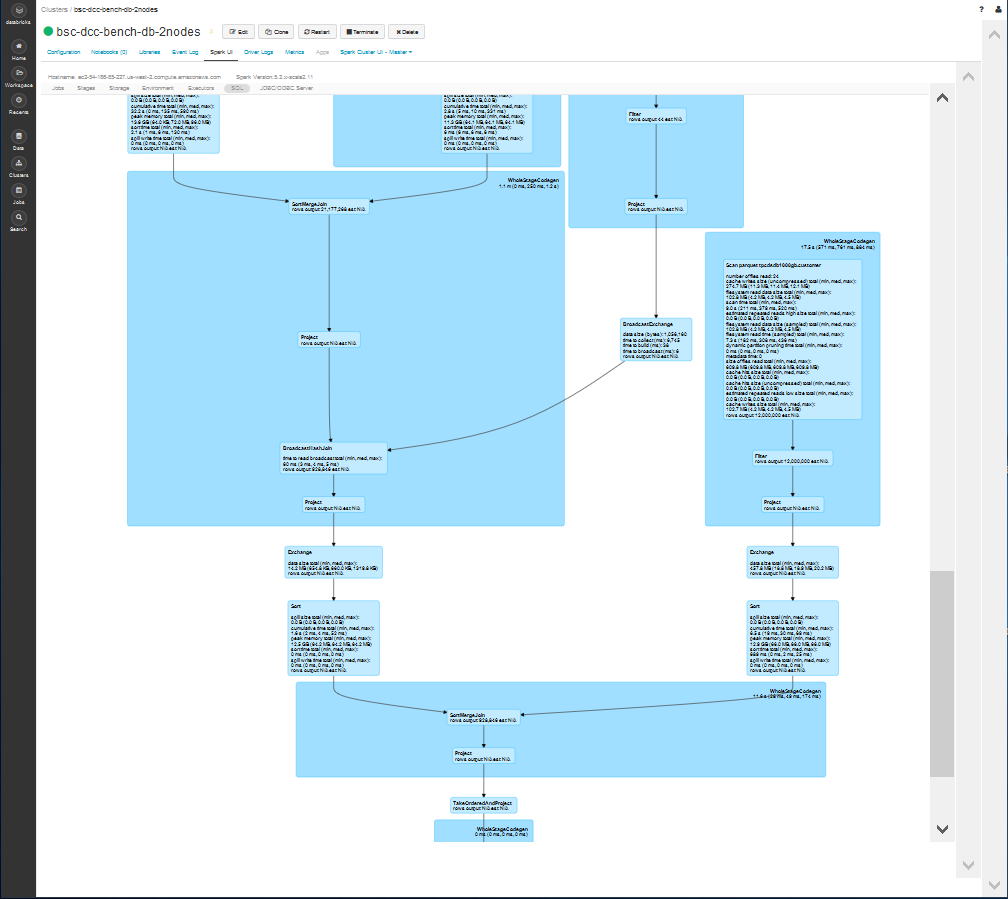
\includegraphics[width=7.0in]{imgs/usability/DatabricksSparkSQLGUI.png}}
   \end{center}
   \caption{Databricks Spark SQL query plan visualization.}
   \label{fig:databricksSparkGUISQL}
\end{figure}

Besides monitoring the progress of query execution, it is desirable to monitor the utilization and the state of computational resources. Databricks incorporates for this task the Ganglia distributed monitoring system and its web GUI, shown in Figure \ref{fig:databricksGanglia}.

\begin{figure}
   \begin{center}
   \scalebox{0.85}{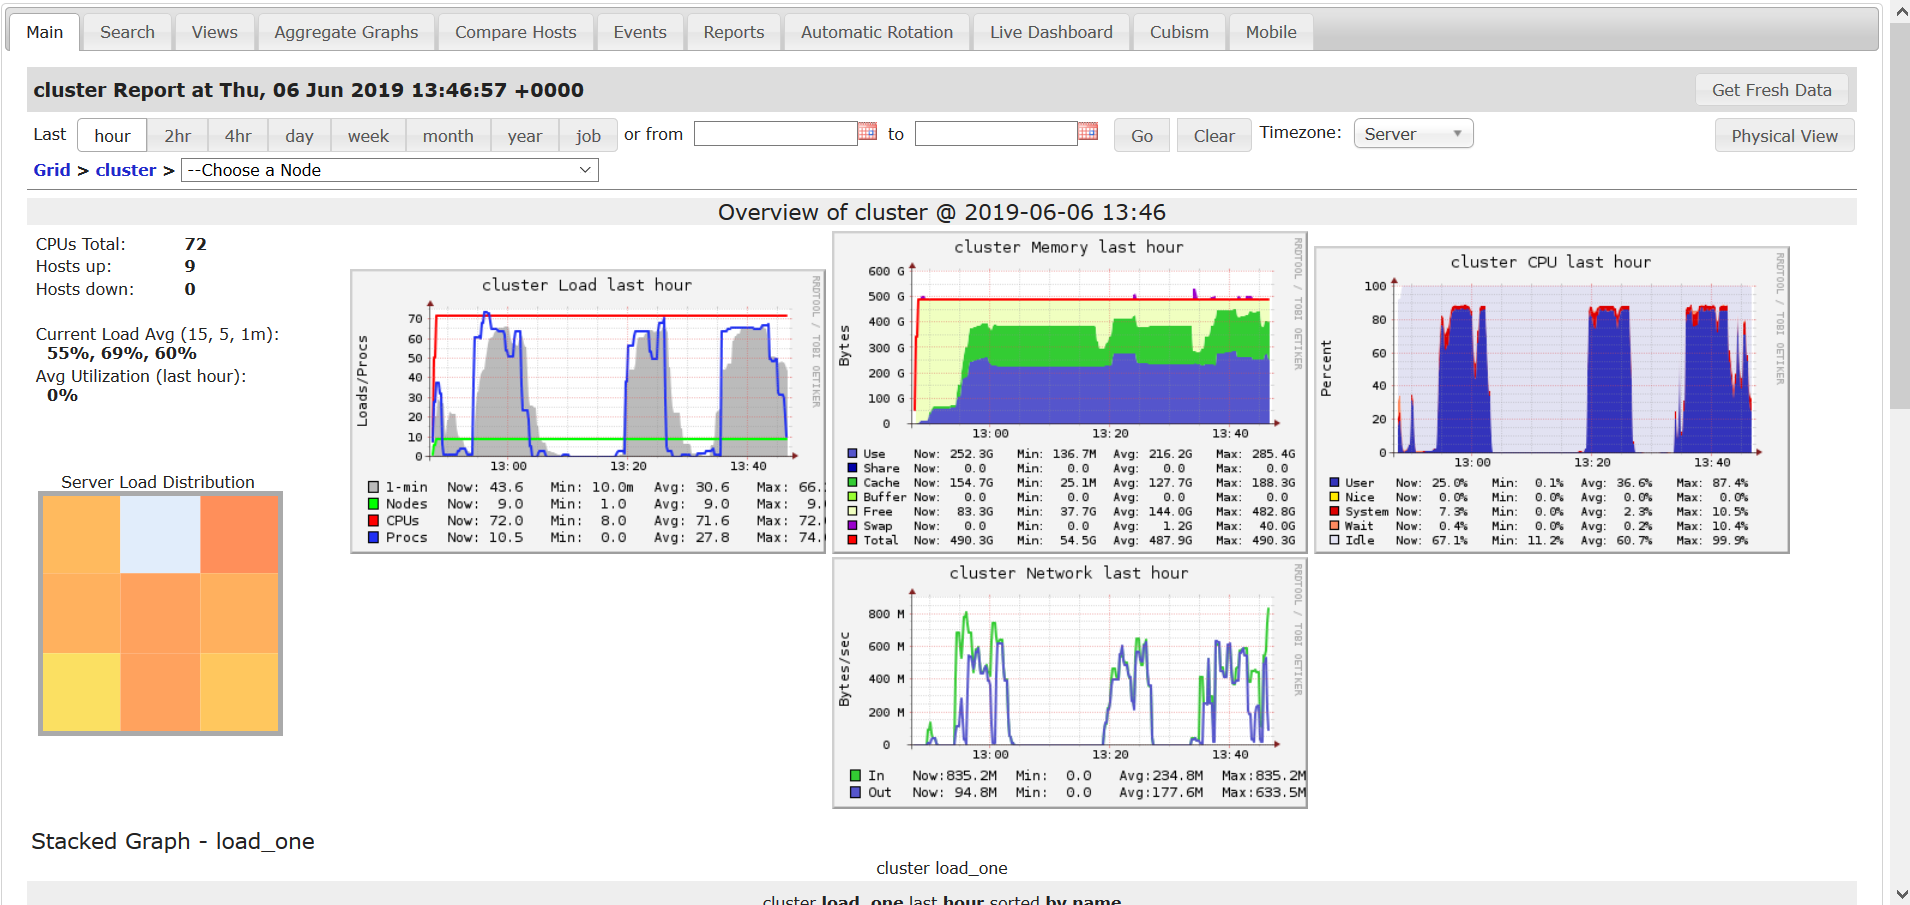
\includegraphics[width=7.0in]{imgs/usability/DatabricksGanglia.png}}
   \end{center}
   \caption{Databricks Ganglia GUI.}
   \label{fig:databricksGanglia}
\end{figure}

It provides aggregate and node-specific metrics related to memory, CPU, and network utilization. Complementing Ganglia, users running Databricks on an AWS EC2 cluster also have at their disposal the CloudWatch monitoring system. We discuss it further in the next subsection in the context of EMR Presto, since both systems do not differ in this regard except for framework-specific metrics. EMR Presto also provides Ganglia and its associated GUI if it is selected at cluster creation time, but it requires setting up an SSH tunnel for access.

\subsubsection{AWS EMR Presto}

EMR Presto provides a web GUI to monitor the activity of the server and visualize the execution of queries. This web GUI, shown in Figure \ref{fig:prestoGUI}, does not require additional configuration to setup, but in order to access it is necessary to establish an SSH tunnel through the appropriate command.

\begin{figure}
   \begin{center}
   \scalebox{0.85}{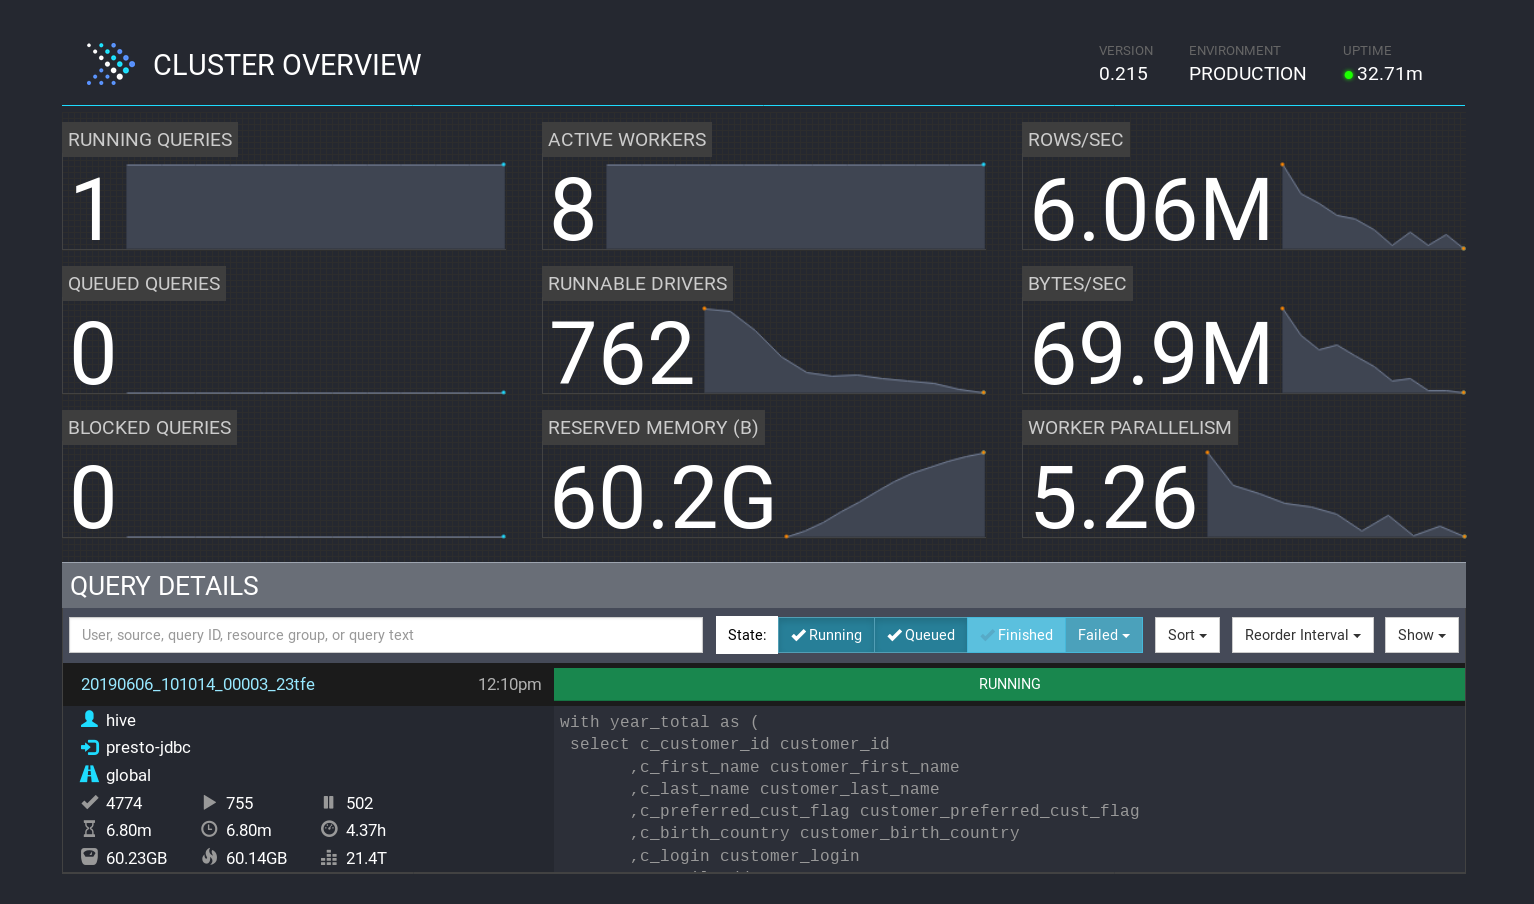
\includegraphics[width=7.0in]{imgs/usability/PrestoGUI.png}}
   \end{center}
   \caption{EMR Presto web GUI.}
   \label{fig:prestoGUI}
\end{figure}

In addition to general information about the state of the cluster and the past and currently executing queries, it is possible to visualize the query evaluation plan used to evaluate a particular query. Figure \ref{fig:prestoLivePlan} provides an example.

\begin{figure}
   \begin{center}
   \scalebox{0.85}{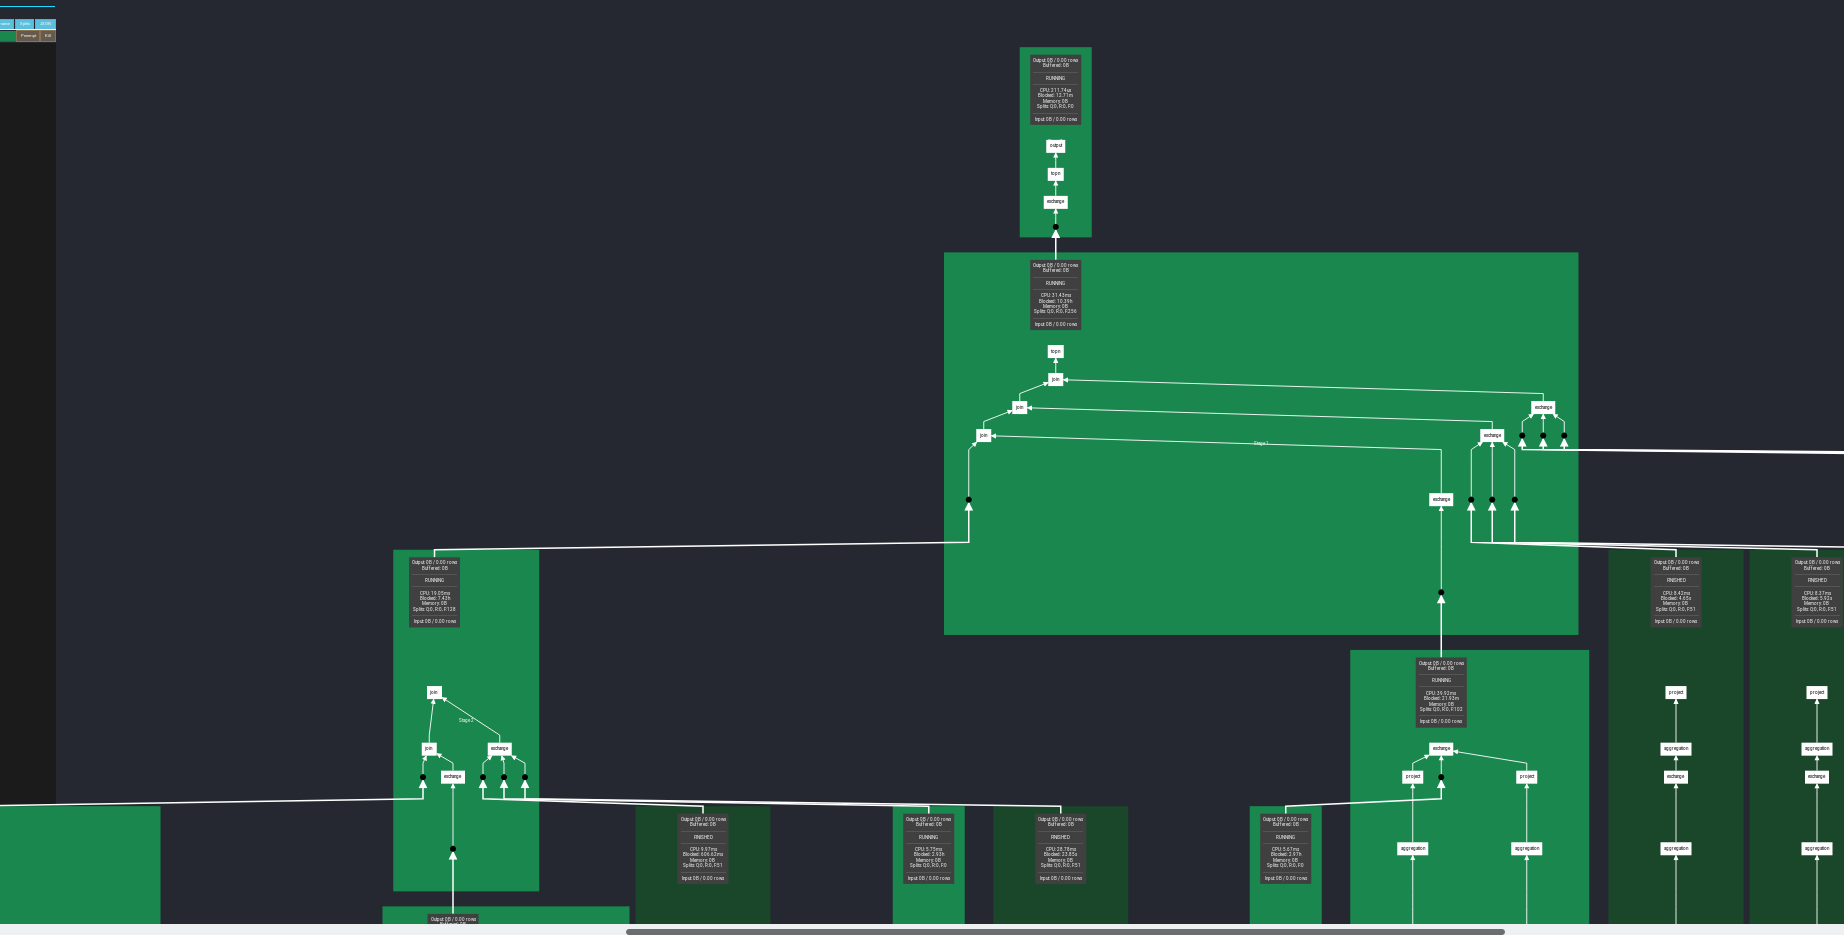
\includegraphics[width=7.0in]{imgs/usability/PrestoLivePlan.png}}
   \end{center}
   \caption{EMR Presto query evaluation plan visualization.}
   \label{fig:prestoLivePlan}
\end{figure}

The user can visualize the query evaluation plan at different zoom levels. Furthermore, the LivePlan feature enables to dynamically visualize how the different stages are completed during the execution of the query. Still the information presented about each stage is somewhat limited in comparison to the Databricks Spark SQL GUI, it would be desirable to view the actual file names used by the scan operators or the attributes used in joins, for example. In addition, it would be convenient to be able to download and subsequently load the execution data and the evaluation plan visualization.

In relation to monitoring resource utilization, EMR Presto employs Ganglia if it is selected at cluster creation time, requiring an SSH tunnel setup to be accessible. In addition, AWS CloudWatch provides a series of metrics related to the EC2 instances that compose the cluster. Some basic metrics are accessible in the main GUI by default, including CPU utilization, network io, disk io, but notably not memory utilization. Additional metrics corresponding to either EMR or the systems that interact with it are made available within CloudWatch, as Figure \ref{fig:cloudWatchaAllMetrics} shows these reach a total of 797 metrics.

\begin{figure}
   \begin{center}
   \scalebox{0.85}{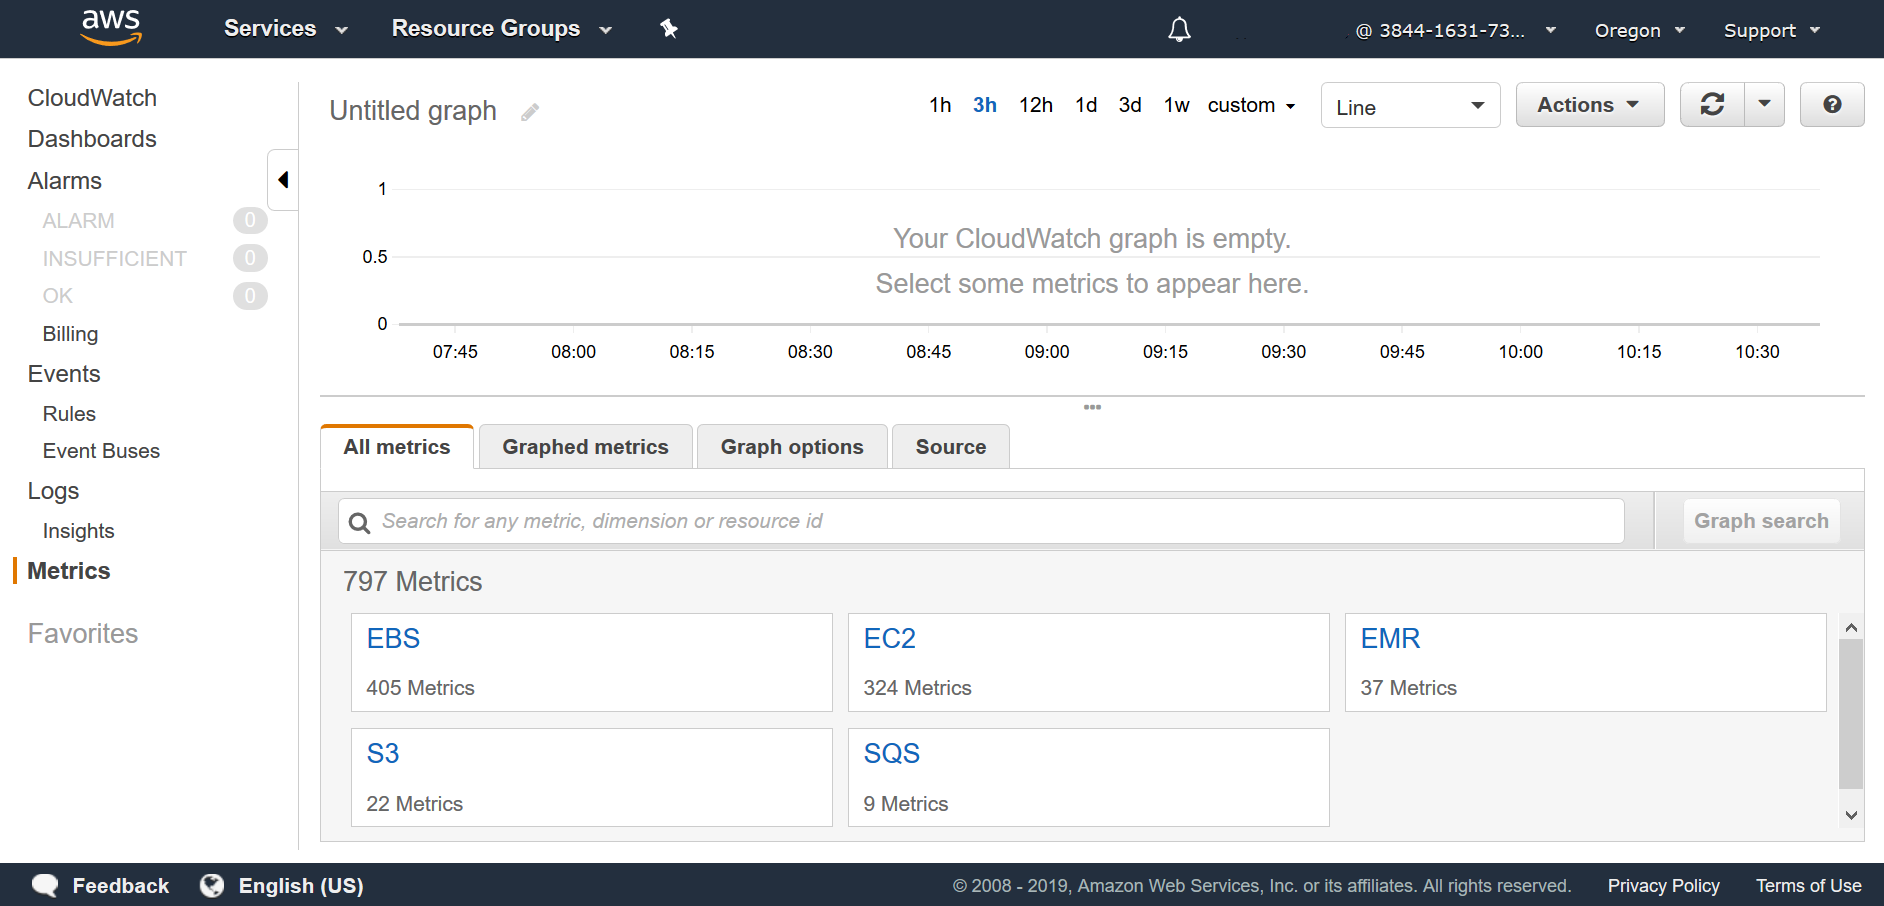
\includegraphics[width=7.0in]{imgs/usability/CloudWatchAllMetrics.png}}
   \end{center}
   \caption{AWS EC2 CloudWatch web GUI.}
   \label{fig:cloudWatchaAllMetrics}
\end{figure}

When using CloudWatch with a Databricks cluster the EBS and EMR metrics do not apply, but the EC2 and S3 metrics are available. Again, both systems use Ganglia with the caveat that it has to be selected in EMR and accessed through an SSH tunnel. Therefore, the resource utilization monitoring capabilities of both Databricks and EMR Presto are essentially equal, with no significant advantage of disadvantage.

